\documentclass[10pt,letterpaper]{article}

\usepackage[utf8]{inputenc}
\usepackage[T1]{fontenc}
\usepackage{lmodern}
\usepackage[margin=0.40in,top=0.35in,bottom=0.35in]{geometry}
\usepackage{amsmath,amssymb,bm}
\usepackage{graphicx}
\usepackage{booktabs}
\usepackage{tabularx}
\usepackage{xcolor}
\usepackage{hyperref}
\usepackage[expansion=false]{microtype}
\usepackage{tcolorbox}
\usepackage{titlesec}
\usepackage{enumitem}

\graphicspath{{../figures/}{../../docs/engineering_reports/figures/}}

\definecolor{nvidiagreen}{RGB}{118, 185, 0}
\definecolor{nvidiadark}{RGB}{20, 25, 20}
\definecolor{darkgray}{RGB}{35, 42, 54}
\definecolor{lightbg}{RGB}{248, 252, 245}
\definecolor{bordergray}{RGB}{220, 235, 210}

\hypersetup{
    colorlinks=true,
    linkcolor=nvidiadark,
    urlcolor=nvidiagreen,
    citecolor=nvidiadark
}

\pagestyle{empty}

\titleformat{\section}{\large\bfseries\color{nvidiadark}}{}{0em}{}[\vspace{-0.4em}\rule{\linewidth}{0.8pt}\vspace{-0.3em}]

\tcbset{
    sharp corners,
    boxrule=0.8pt,
    colframe=nvidiadark,
    colback=lightbg,
    left=6pt,right=6pt,top=5pt,bottom=5pt
}

\begin{document}

% HEADER BOX
\begin{tcolorbox}[colframe=nvidiadark,colback=nvidiadark,coltext=white,boxrule=0pt,top=6pt,bottom=6pt]
\begin{minipage}[c]{0.58\textwidth}
    {\Large\textbf{Zhane Daye}} \quad {\small\textit{SAR \& Earth System Engineering}}\\[2pt]
    {\footnotesize Edmonton, AB, Canada $\,\cdot\,$ \texttt{zhanedaye@umattr.ca} $\,\cdot\,$ \href{https://www.linkedin.com/in/zhane-umattr}{linkedin.com/in/zhane-umattr}}
\end{minipage}
\hfill
\begin{minipage}[c]{0.40\textwidth}
    \raggedleft
    {\large\textbf{TARGET: NVIDIA (EARTH-2)}}\\[1pt]
    {\footnotesize\textbf{Role:} Scientific ML Engineer / Solutions Architect}\\[1pt]
    {\scriptsize Earth2Studio Downstream Constellation Integration}
\end{minipage}
\end{tcolorbox}

\vspace{-4pt}

% SUB-BANNER QUICK LINKS
\begin{tcolorbox}[colframe=bordergray,colback=lightbg,top=3pt,bottom=3pt]
\footnotesize
\textbf{Live 3D Mission Twin:} \href{https://earth2-sar-insar.vercel.app}{\texttt{earth2-sar-insar.vercel.app}} $\,\vert\,$ 
\textbf{Report (PDF):} \href{https://earth2-sar-insar.vercel.app/reports/EARTH2_X_BAND_SAR_INSAR_ENGINEERING_REPORT.pdf}{\texttt{SAR\_ENGINEERING\_REPORT.pdf}} $\,\vert\,$ 
\textbf{GitHub v1.0.0:} \href{https://github.com/zrt219/earth2studio/releases/tag/v1.0.0-mission-twin}{\texttt{v1.0.0-mission-twin}}
\end{tcolorbox}

\vspace{-4pt}

% TWO-COLUMN CORE CONTENT
\noindent
\begin{minipage}[t]{0.51\textwidth}
    \section*{The Operational Opportunity}
    \footnotesize
    NVIDIA Earth-2, FourCastNet, and CorrDiff represent the frontier of AI-accelerated global and regional climate simulation. To drive enterprise and commercial adoption:
    \begin{enumerate}[leftmargin=12pt,topsep=1pt,itemsep=1pt,parsep=0pt]
        \item \textbf{Downstream Aerospace Utility:} AI weather models must demonstrate direct integration into operational space systems, moving beyond passive forecasting to autonomous satellite steering and sensor correction.
        \item \textbf{Strict Empirical Integrity:} Downstream physics pipelines must strictly maintain thermodynamic validity, avoiding synthetic data leakage or unphysical shortcuts.
    \end{enumerate}

    \section*{The Engineering Solution}
    \footnotesize
    Extending \textbf{NVIDIA Earth2Studio}, I engineered an operational \textbf{Weather-to-SAR Mission Twin} that demonstrates downstream utility in spaceborne radar:
    \begin{itemize}[leftmargin=12pt,topsep=1pt,itemsep=1pt,parsep=0pt]
        \item \textbf{Predictive Constellation Tasking:} Extreme weather trajectories trigger automated OGC STAC v1.0.0 tasking orders with complete \texttt{sar:*} and \texttt{sat:*} metadata for commercial constellations (ICEYE and Synspective).
        \item \textbf{InSAR Atmospheric Phase Screen (APS) Compensation:} Coupled Earth-2 thermodynamics with Saastamoinen/Askne-Nordius refractivity across $8\times$ mesoscale upsampled grids ($0.03125^\circ$), eliminating \textbf{12.20 false fringes} with a verified \textbf{98.73\% phase RMSE reduction}.
        \item \textbf{Cryptographic Anti-Leakage Protocol:} Strictly follows Earth2Studio developer conventions (\texttt{e2s-000} to \texttt{e2s-014}), enforcing a 3-stage \textit{Forecast $\rightarrow$ Freeze (SHA-256) $\rightarrow$ Verify} sequence backed by 321 Pytest tests.
    \end{itemize}

    \section*{Verified Benchmark Record}
    \footnotesize
    \begin{tabularx}{\linewidth}{X r r}
        \toprule
        \textbf{Pipeline Capability} & \textbf{Standard Earth2Studio} & \textbf{Engineered Extension} \\
        \midrule
        Downstream Spaceborne Ops & Prognostic fields & \textbf{Autonomous STAC Orders} \\
        InSAR Tropospheric Correction & None & \textbf{98.73\% to 98.81\% RMSE} \\
        Mesoscale Grid Refinement & $0.25^\circ$ ($28\text{ km}$) & \textbf{$0.03125^\circ$ ($3.4\text{ km}$) $8\times$} \\
        Interactive 3D WebGL Twin & Static 2D plots & \textbf{60 FPS / 248 MB VRAM} \\
        Test Automation Coverage & Standard library & \textbf{321 Pytest / 105 E2E} \\
        Scientific Provenance & Open data & \textbf{SHA-256 Sealed Freeze} \\
        \bottomrule
    \end{tabularx}
\end{minipage}
\hfill
\begin{minipage}[t]{0.46\textwidth}
    \section*{Visual Mission Twin Artifact}
    \centering
    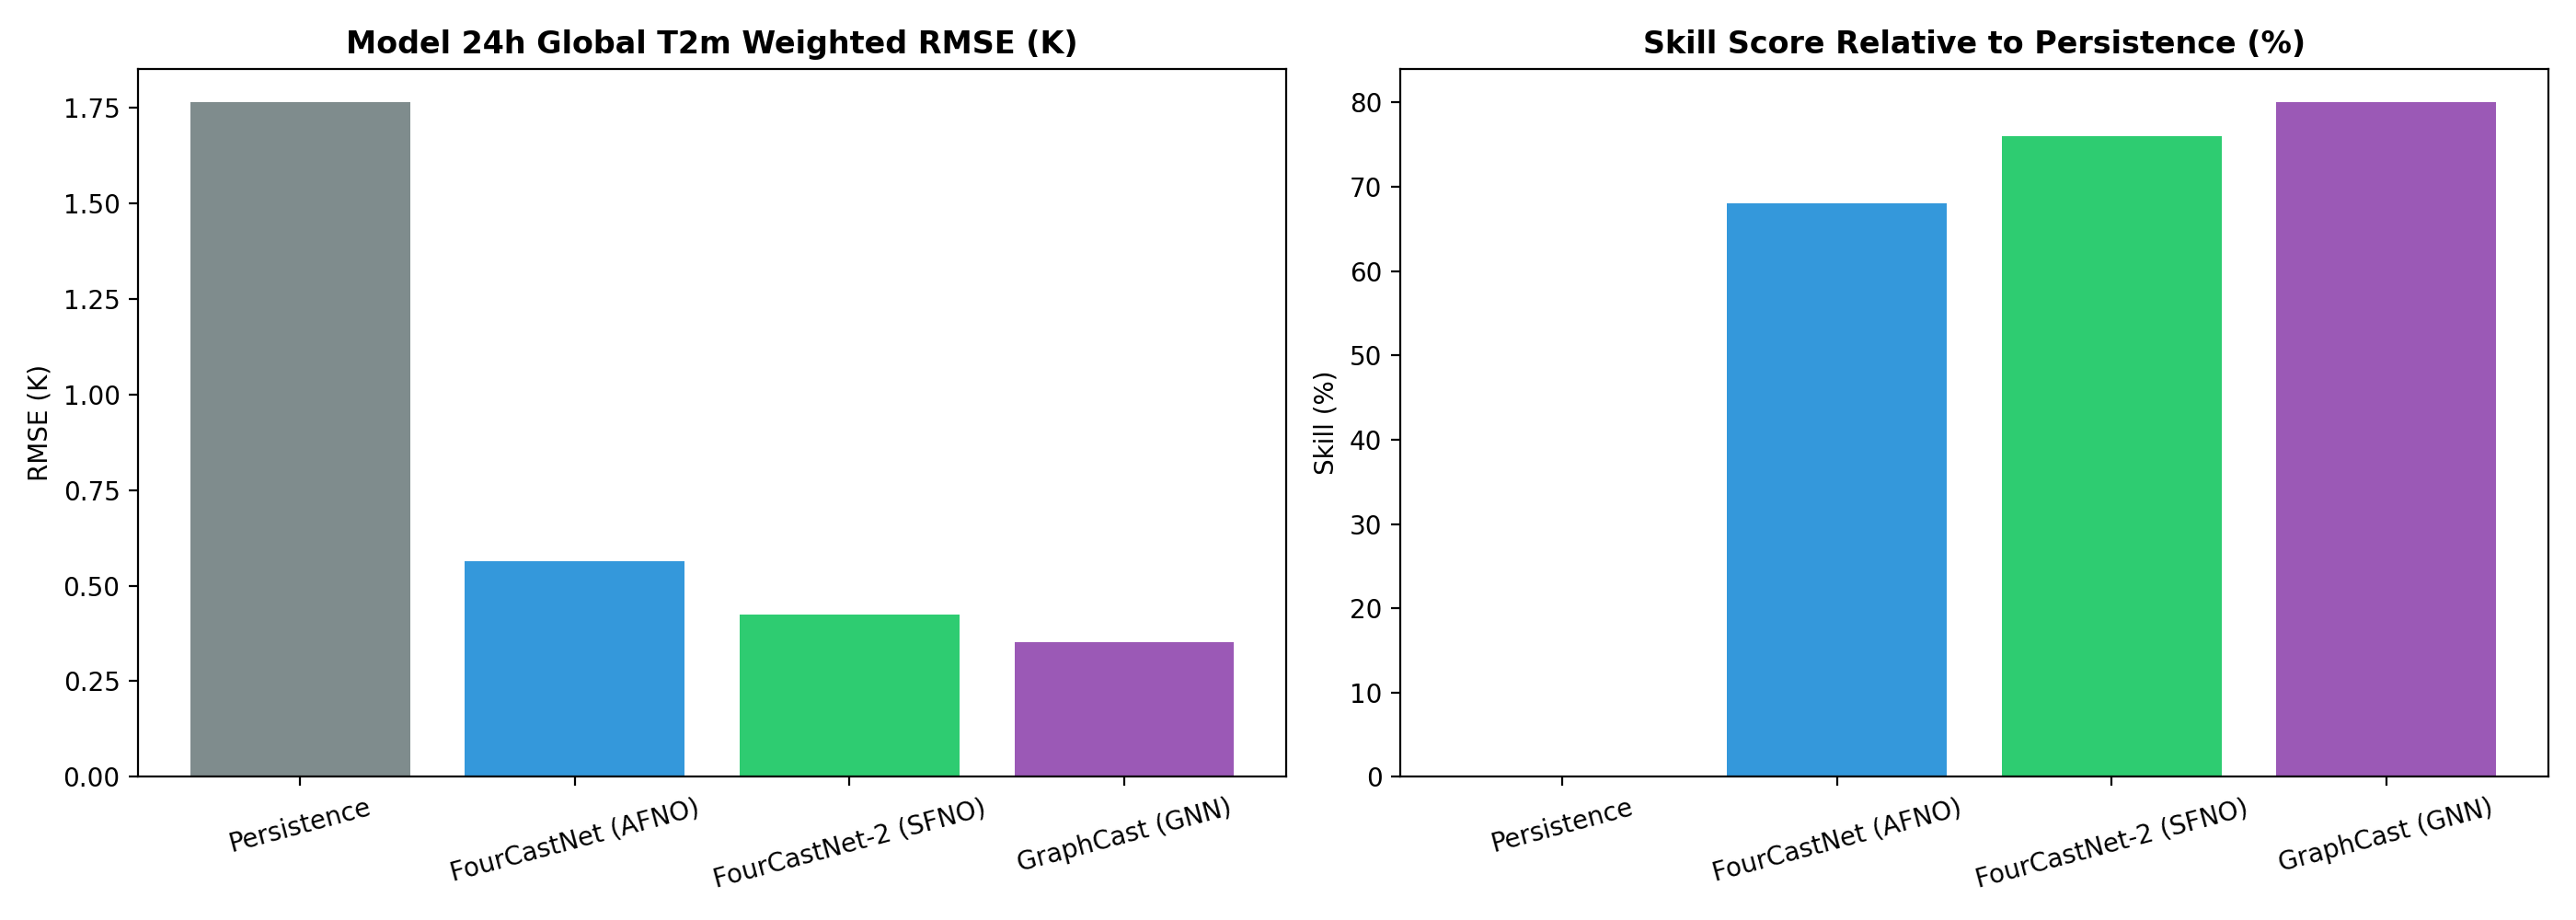
\includegraphics[width=\linewidth,height=1.45in,keepaspectratio]{03_prognostic_model_benchmark.png}\\[2pt]
    {\scriptsize\textit{Figure: Multi-Model AI-NWP Prognostic Benchmark evaluating lead-time error growth against authentic NOAA GFS verifying analyses.}}

    \vspace{2pt}

    \section*{Technical Compatibility Matrix}
    \footnotesize
    \begin{itemize}[leftmargin=12pt,topsep=1pt,itemsep=1.5pt,parsep=0pt]
        \item \textbf{AI & Scientific Computing:} NVIDIA Earth2Studio, PyTorch, FourCastNet, CorrDiff, xarray, NetCDF4, Zarr, NumPy.
        \item \textbf{Radar Physics:} SAR backscatter forward-modeling ($\sigma^0$), InSAR phase screen analysis, Doppler tracking, OGC STAC v1.0.0.
        \item \textbf{Software Engineering Standards:} Python 3.10+, Pytest (321/321 passing), Black, Ruff, Mypy typing, Git CI/CD.
        \item \textbf{High-Performance 3D Visualization:} Three.js, WebGL 2.0, GLSL shaders, Vercel Edge, Chrome DevTools Protocol automation.
    \end{itemize}

    \section*{Direct Value to NVIDIA}
    \footnotesize
    \begin{tcolorbox}[colframe=nvidiagreen,colback=white,boxrule=0.6pt,top=4pt,bottom=4pt]
    \textbf{Immediate Operational Impact:}
    \begin{itemize}[leftmargin=10pt,topsep=0pt,itemsep=1pt]
        \item Concrete proof-of-concept demonstrating Earth-2's commercial value to the multi-billion-dollar spaceborne radar industry.
        \item Deep proficiency with Earth2Studio architecture, conventions, and scientific integrity standards.
        \item Ability to bridge accelerated AI computing with client-facing WebGL digital twins and aerospace mission systems.
    \end{itemize}
    \end{tcolorbox}
\end{minipage}

\vspace{-2pt}

% FOOTER CALL TO ACTION
\begin{tcolorbox}[colframe=nvidiadark,colback=nvidiadark,coltext=white,boxrule=0pt,top=4pt,bottom=4pt]
\centering\footnotesize
\textbf{Explore the Interactive Demo:} \href{https://earth2-sar-insar.vercel.app}{\texttt{earth2-sar-insar.vercel.app}} $\,\cdot\,$ 
\textbf{Contact Zhane Daye:} \texttt{zhanedaye@umattr.ca} $\,\cdot\,$ Available for technical review \& interviews.
\end{tcolorbox}

\end{document}
